
\chapter{Static gestures recognition}

As was already mentioned, the detected gestures can be divided into two groups: static gestures and dynamic gestures.
The static gestures can be understood as a chosen position and orientation of the fingers and hand in a single moment, while dynamic gestures are defined as a movement of the hand and fingers in time. 
The problem of recognition of those gestures is a subject of following chapter. 
Firstly, the proposed approach is presented, followed by the introduction to the evaluation scheme. 
In last section, the performed experiments are descriebed, which were used to examine the effectiveness of proposed static gesture recognition approach.

\section{Proposed methods}

The static gesture recognition problem can be stated as a problem invariant to time.
That means that for each detected hand, the position and orientation can be treated as a new data uncorrelated to previously classified data.
While this assumption means that one can easily generate multiple samples from the sensors in short time, it also gives an opportunity to look at the static gesture recognition problem as a problem of classification.

While for most 2D gesture recognition problems simple classification algorithms seems to work well enough, the 3D data is more complication to model by the set of features and finally successfully label.
While dealing with 3D data, the position and orientation of hand can be easily affected by the height of the hand above the sensor or small change in the orientation of the hand with respect to the sensor's coordinate system. 
It is intuitively understood, that the system should recognize those gestures as the one as they are similar.
To meet those requirement, one need to define what is meant by the ``small'' change in orientation resulting in treating the static gestures as the same.

\begin{figure}[htb]
\centering
 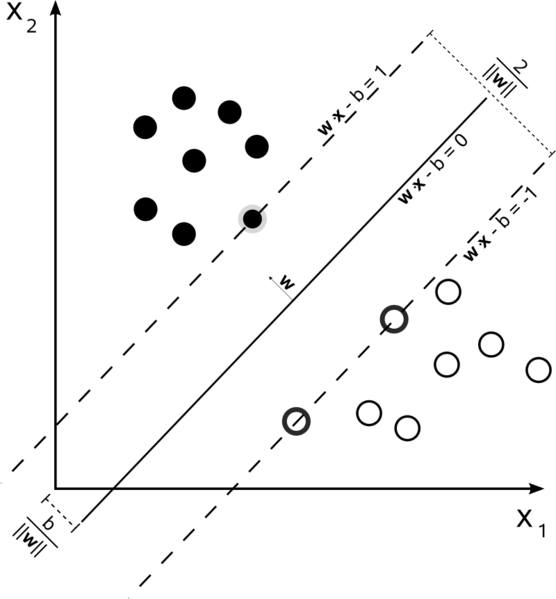
\includegraphics[width=0.6\columnwidth]{figures/SVM.png}
 \caption[]{SVM is a technique searching for the hyperplane that maximizes the margin between classes\footnotemark}
 \label{svmmargin}
\end{figure}



To meet those requirements, the Support Vector Machines \cite{Cortes:SVM} were used as a classification algorithm.
The SVMs were chosen as there exist a solid mathematical background supporting the simple idea of maximalizing the margin between classes.
Moreover, the SVMs were chosen also because of the popularity due to the open-source library libSVM \cite{libSVM}, which contains the multiple platform SVM implementation.
It is worth noticing that in original work, SVMs were used only to classify between two classes, but the idea was expanded to utilize the one-vs-all scheme allowing to classify multiple class sets.
The efficiency of SVMs depends on correctly choosing the kernel function used to map the separation problem into higher-dimension with expectation to achieve problem easier to solve.
The typical kernel functions:
\begin{itemize}
\item linear: $K(x_i, x_j) = x_i^Tx_j$.
\item polynomial: $K(x_i, x_j) = (\gamma x_i^Tx_j + r)^d, \gamma > 0$.
\item radial basis function (RBF): $K(x_i, x_j) = exp(-\gamma ||x_i - x_j||^2), \gamma > 0$.
\item sigmoid: $K(x_i, x_j) = tanh(\gamma x_i^Tx_j+r)$.
\end{itemize}
where $\gamma$, $r$, and $d$ are kernel parameters. According to the authors of the library, linear kernels should be used for linearly separable problems, while RBF kernel is the most versatile one.

\footnotetext{\url{http://en.wikipedia.org/wiki/File:Svm_max_sep_hyperplane_with_margin.png}}

The problem of classification assumes that each sample consists of set of features, which describe this sample and can be used to distinguish it from the other samples.
Additionally, each sample has a known or unknown label, which defined the membership of sample to the class. 
The samples with the known labels can be used to train the classification system to compute the membership to the classes for the samples. 
The computation is performed on previously mentioned sets of features.

In application of gesture recognition the classification be divided into two flows: the training part and the recognition part. 
In training part, the library will be provided with the samples of static gestures with known correspondences to the static gesture classes. 
From those samples, the sets of features are computed, which are used to train the classifier.
The recognition part assumes to have trained classifier. 
The recognition part is provided with samples static gestures without labels. 
For each sample the sets of features are computed and then given as input to the trained classifier.
The classifier returns the information of the gesture's class membership (label) of each sample.

In case of library, it is assumed that the learning process can be done offline, while strict online requirements has to be met in recognition part. 
To meet those requirements the Support Vector Machine is introduced\cite{Cortes:SVM}. 
The SVM classification is commonly used technique in multiple areas of research as biology, robotics or IT for solving data classification problems.
Additional advantage of the SVM is possibility to use C++ library libSVM \cite{libSVM}, which provides an easy interface to utilize this classification methods in different problems.

\begin{figure}[htb]
\centering
 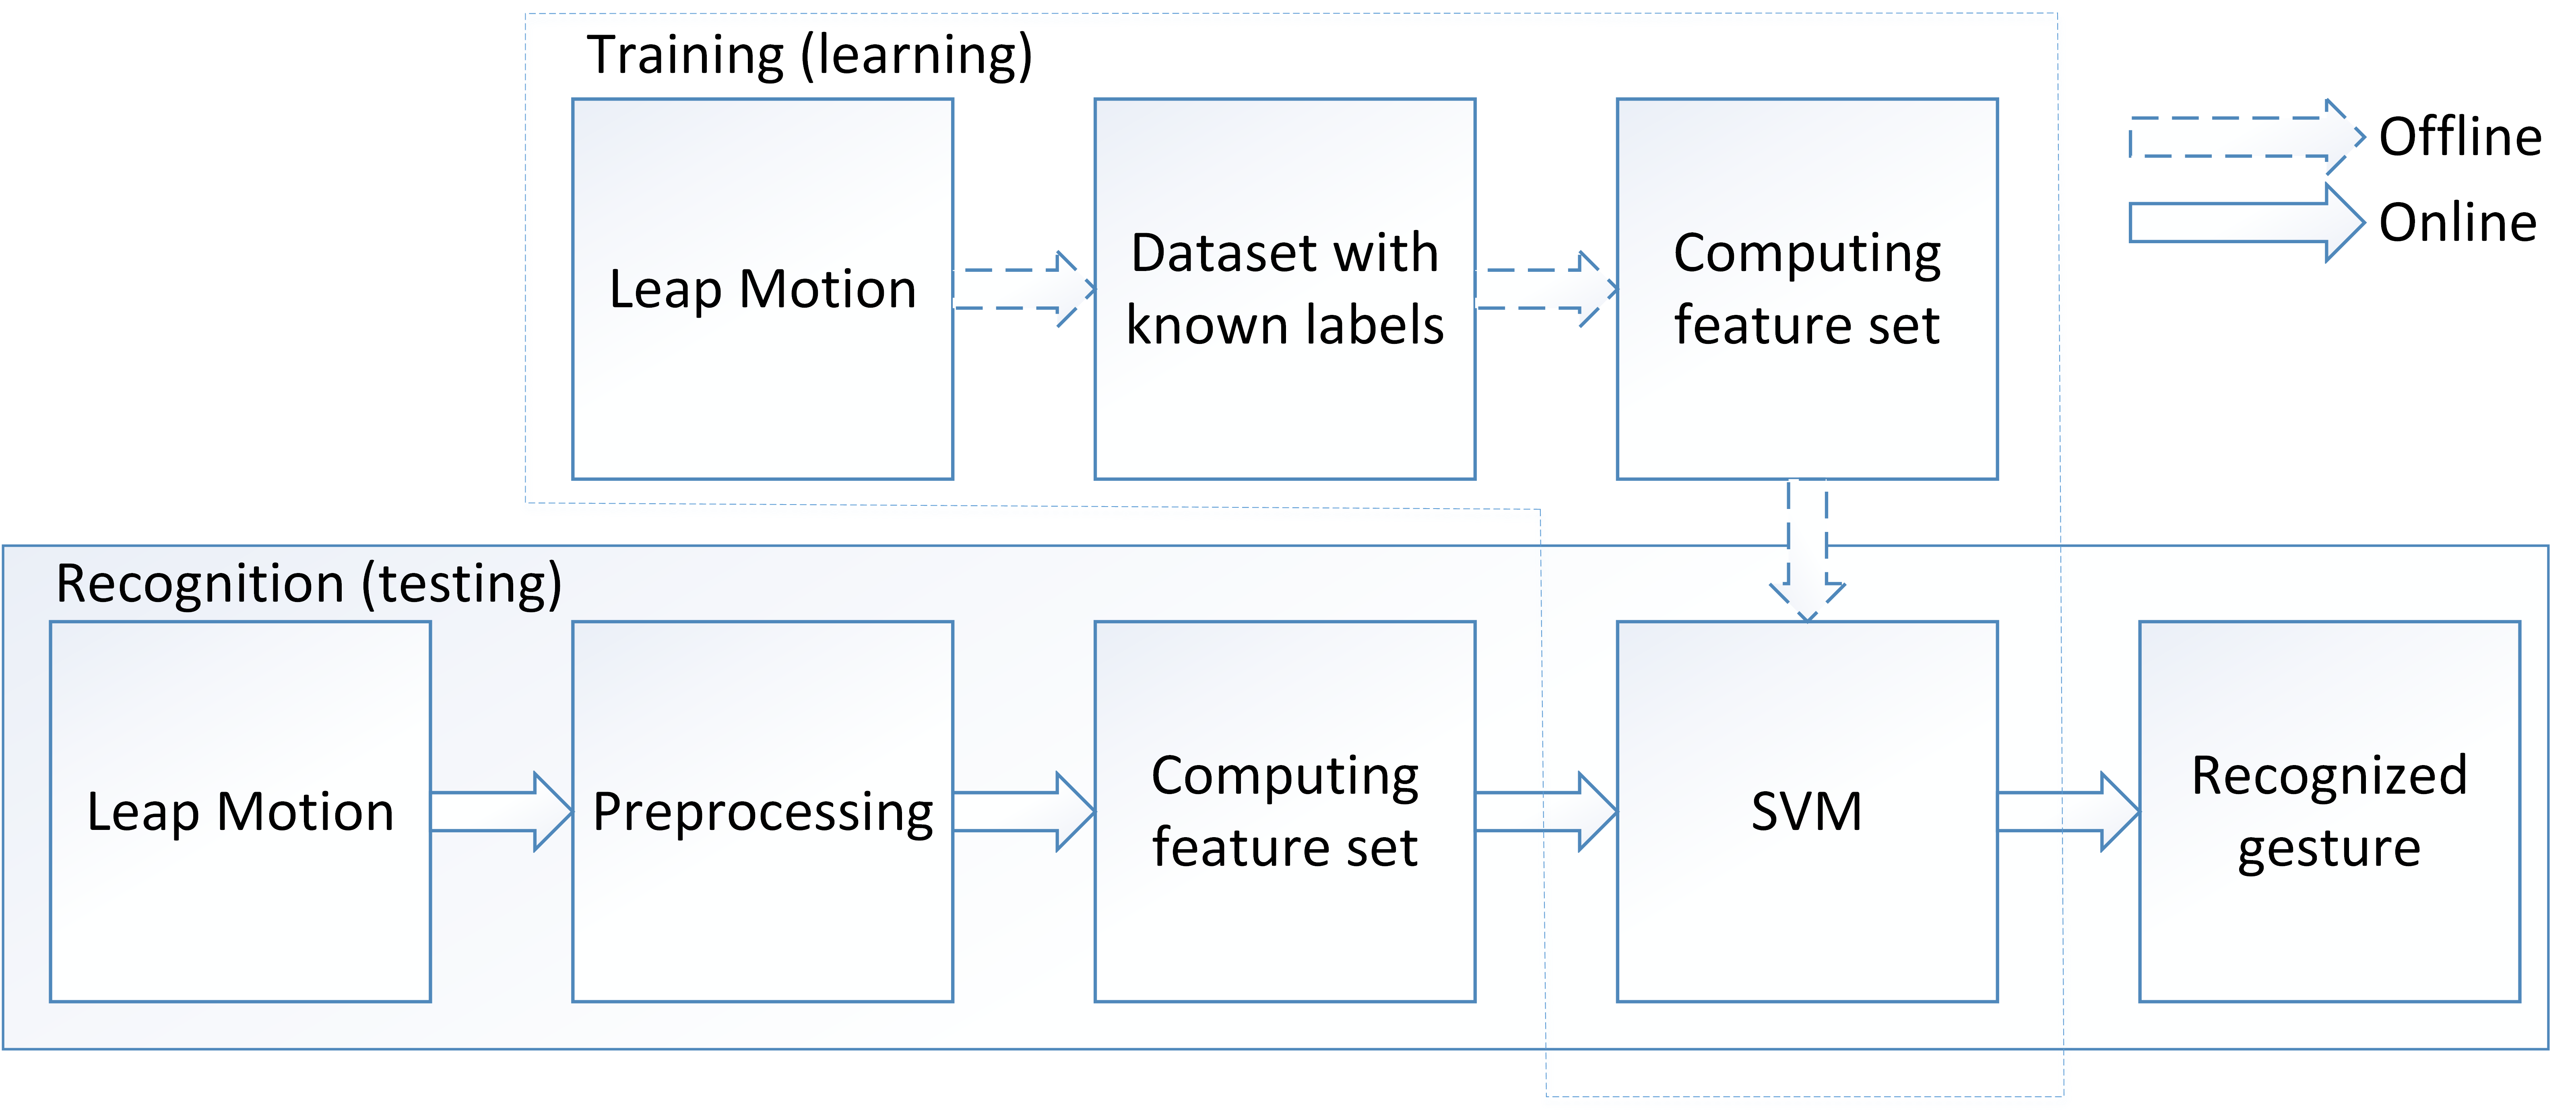
\includegraphics[width=1\columnwidth]{figures/StaticGestures.png}
 \caption[]{Proposed solution blocks for learning and recognition parts of static gestures recognition problem}
 \label{staticsol}
\end{figure}


While presented approach can be treated as state-of-the-art approach it still cannot be used without defining proper feature sets for gesture recognition.
The naive solution would be to use the raw data from Leap motion sensor as the feature set.
This solution was tested, but provided poor results as the proposed features were dependent on the position, orientation and scale of hand. 
Even small movement in any direction meant problems with stable recognition. 
The theoretical literature suggests to compute a set of features invariant to wanted transformations, which can allow to fully distinguish between different classes.
Unfortunately, there are not available propositions to feature sets when it comes to the gesture recognition using the data even similar to the data provided by the Leap Motion sensor.
Seeking right feature is a task undertaken in experimental section~\ref{static:exp}.

To sum up, the static gesture processing flow is presented at fig.~\ref{staticsol}. In training part, the data from Leap Motion is preprocessed, the feature sets are computed and the data is used to train SVM classifier.
In recognition part, the data is also preprocessed and described by the feature sets, but the knowledge of the label comes from the already trained SVM classifier.


\section{Evaluation methodology}

\subsection{Assumptions}
To provide user with library working in different conditions, it was assumed that the gesture is treated as the same one independently with respect to the translation, rotation and scale of the hand. 
This assumption means that the static gesture rotated by unknown angles, translated in sensor coordinate system and also with different hand sizes should still be recognized as the same gesture.
Invariance to the rotation, translation and scale poses a great challenge to the recognition, but allows the future users of API to fully utilize the feasibility of the library.
It is worth mentioning that, it does not reduce the possible applications of the library, as an assignment of static gesture to already defined class allows to find the transformation between the model of the class and observed gesture.


\subsection{Recorded datasets}

To propose and test the quality of the features twelve static gestures were chosen:
\begin{enumerate}
\item the peace sign,
\item a fist,
\item full hand with space between each finger,
\item American Sign Language: ``I love you'' sign,
\item sign ``gun'' created by putting thumb and forefinger up, while holding the rest fingers in a fist,
\item all fingers in a fist with exception of thumb, which is up,
\item the sign X made with the forefingers of both hands,
\item the sing ``Time'' used e.g. by coaches in basketball games.
\item sign simulating rotating a knob by two fingers,
\item sign simulating rotating a knob by five fingers.
\end{enumerate} 

\begin{figure}[htb]
\centering
 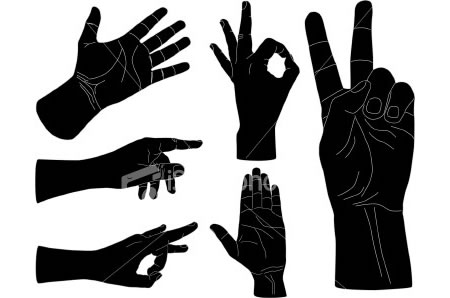
\includegraphics[width=1.0\columnwidth]{figures/static_gestures.png}
 \caption{Recorded static gestures used for evaulation}
 \label{staticgesturesdata}
\end{figure}


The gestures are also presented at fig.~\ref{staticgesturesdata}.


The sample data of each gestures were recorded using the continuous mode of recording, while moving the hands in different directions and changing the orientation of the hands. 
For each of the proposed gestures, each author recorded approximately 1000 samples.

Having samples with known labels, the whole dataset was separated into training and testing sets in relation $2:1$. 
For the training, the k-fold cross-validation (CV) scheme was used, which searches for optimal $C$ and $\gamma$ parameters trying to prevent the algorithm from over-fitting the training data.
This method is used to find the optimal parameters of the classification system, while estimating the performance on the data not used in the training part. 
In standard version of the method, the gathered data is divided into two sets: one containing k-1 parts of the data, the other 1 part of the data. 
The first is used to train the classification system, while the rest of the gathered data is used to estimate the performance. 
The performance is estimated by calculating the number of cases when the classification system returned a label which matched already known label. 
The percent of correctly recognized labels to the total size of the testing set is known as recognition rate.


\section{Experiments}
\label{static:exp}

Firstly, the experiments to find the proper set of features were conducted. The first proposed vector of features consisted of:
\begin{itemize}
\item number of fingers in frame,
\item the euclidean distance between consecutive finger's tips,
\item the absolute angles between consecutive fingers.
\end{itemize} 

While this feature set did not take into account the relative position of fingers to the hand, the second and third feature set were introduced.
The second feature set is a first feature set extended by the distances between consecutive finger tips and the position of the hand's palm.
The third feature set contains features from second feature set extended by the five angles between fingers and normal of hand's palm.
Those, 3 proposed feature sets were firstly tested on all $10$ recorded static gestures.
The firstly tested set of all static gestures contained gestures, which were undistinguishable for the Leap Motion, because they did not take into account the way how the Leap Motion works. 
For gestures like fist or 'X' the recorded data contained almost no information how to classify those gestures.
That's why the experiments were repeated on the five gestures, which could be easily distinguish using the data provided by Leap Motion. 
For this experiment the gestures peace, hand, ''I love you'', fist with thump up and rotating knob by 5 fingers were chosen.
The results achieved by those methods are presented in the table~\ref{staticfeat}.

\begin{table}[htp!]
	\label{staticfeat}
	\caption{Results obtained by experimental feature sets by the libSVM library}
    \begin{tabular}{|c|c|c|c|c|}
    \hline
    ~                                                   & 5 gestures, CV & 5 gestures, test set & 10 gestures, CV  & 10 gestures, test set \\ \hline
    feature set 1                     & 87.072\% & 87.943\% & 69.987\% & 68.422\%   \\ \hline
    feature set 2                     & 87.072\% & 87.943\% & 69.987\% & 68.422\%          \\ \hline
    feature set 3                     & 87.072\% & 87.943\% & 69.987\% & 68.422\%           \\ \hline
    feature set 4                     & 81.150\% & 80.998\% & 68.438\% & 68.630\%          \\ \hline
    feature set 5                     & 86.544\% & 85.075\% & 77.101\% & 77.518\%          \\ \hline
    feature set 6                     & 92.762\% & 93.096\% & 80.543\% & 81.235\%           \\ \hline
    \end{tabular}
\end{table}

For problem of recognition of 5 gestures, 3 first feature sets resulted in over $87$\% recognition rate on testing sets, which was believed to be a good result.
The same tests for problem of recognition of 10 gestures resulted in lower recognition rates.
For feature sets 1-3 the recognition rate was below $70$\%, which could be unsatisfying from the perspective of the purpose of the application.
The low recognition rate was analysed and revealed that the fingers are numbered accordingly to the position in Z axis of the tip of the finger.
This means that when fingers' tips are approximately on the same position in Z axis, the numbering can change rapidly and proposed features are compared between different fingers.
To achieve features that would be invariant to the numbering of the fingers, the feature set was slightly modified.
Instead of containing the absolute angles and distances between consecutive fingers, it was proposed to contain the five greatest values of angles and five greatest values of distances between all combinations of finger pairings.
The same sorting approach was used for the angles and distances between fingers and hand's palm.
The feature sets 1, 2, 3 with sorting scheme were respectively called feature sets 4, 5, 6.
Again, the same dataset with 5 and 10 gestures was used to evaluate those methods. 
The results are yet again presented in table~\ref{staticfeat}.
This approach was tested on the same training set and allowed to increase the recognition rate.
The best results in both tasks were achieved in case of feature sets 6.
The simple alleviation of finger numbering problem allowed to top the previous results with recognition rates $93.096\%$ for 5 gesture problem and $81.235\%$ for 10 gesture problem in case of feature set 6. 

\begin{table}[htp!]
\begin{center}
	\label{staticfeatlin}
	\caption{Results obtained by experimental feature sets by the libLinear library}
    \begin{tabular}{|c|c|c|c|c|}
    \hline
    ~                                                   & 5 gestures, CV & 5 gestures, test set & 10 gestures, CV  & 10 gestures, test set \\ \hline
    feature set 1                     & 78.282\% & 78.283\%  & 50.596\% & 50.593\% \\ \hline
    feature set 2                     & 78.282\% & 78.283\%  & 50.596\% & 50.593\% \\ \hline
    feature set 3                     & 78.282\% & 78.283\%  & 50.596\% & 50.593\% \\ \hline
    feature set 4                     & 78.205\% & 78.242\%  & 50.658\% & 50.575\% \\ \hline
    feature set 5                     & 79.527\% & 79.502\%  & 55.284\% & 55.263\% \\ \hline
    feature set 6                     & 88.0756\% & 88.138\% & 64.747\% & 64.830\% \\ \hline
    \end{tabular}
    \end{center}
\end{table}

While using more data and longer feature sets usually allows to achieve better results, it is worth to notice the growth of training time of classification technique. 
In case of $5000$ training samples the typical training process of radial SVM took approximately 12 hours on standard desktop PC. 
This computing time can be unacceptable by the users of the library, so the test with another SVM library libLinear~\cite{libLinear} was performed. 
The libLinear's implementation of SVM utilizes the linear kernels, which are useful for large data training sets with multiple number of features. 
This library reduced the training time to about 5 seconds.
Again, the same tests as for the libSVM were performed to compare both approaches.
All achieved results are presented in tab.~\ref{staticfeatlin}.
For the 5 gesture case, the libLinear achieved 88.138\% on testing set while using feature set 6 compared to the 93.096\% achieved by libSVM in the same condition.
In this case, the libLinear might be good choice as the recognition rate different is about 5\%.
For 10 gesture case, libLinear achieved 64.830\% compared to 81.235\% by LibSVM, which is a significantly lower.
It's up to user to decide, which library to use, but in most recognition taks applications the library can be learnt offline and only used online.
That is why, the SVM with RBF kernels is a recommended choice in gesture recognition task.

From the results obtained by the libSVM and libLinear on different feature sets, the feature set 6 was chosen as the one yielding the best results and used in further analysis.


Another factor, that might have an influence on the results is the preprocessing part, which should allow to partially remove noise from the data and thus increase the recognition rate. 
The preprocessing operates in the window of hands poses recorded over time, which size can be modified. 
The typical library usage allowed to gather data with $60Hz$, while it is assumed that the recognition can be performed with lower framerate. The difference can be efficiently used by defining the appropriate preprocessing window.
For these reason, the experiments with no preprocessing and preprocessing with width size equal to 5, 10, 15, 20, 30 were performed and the influence on the recognition rate was examined.
The results are presented in tab.~\ref{staticpre}.
The achieved results confirm the need and importance of proper data preparation in task of data classification.
For gesture recognition task containing 5 gesture poses, preprocessing allowed to increase the recognition rate from 93.096\% to over 99\% for window sizes equal or wider than 15. 
In task of correctly detecting 10 gestures, the preprocessing allowed to increase recognition rate from 81.235\% to over 84\% for windows sizes equal or wider than 10.
From those results, the preprocessing width of 10 was chosen as the one allowing to significantly improve recognition rate in almost any possible application of the library.
The preprocessing of width 10 was used for further experiments.

\begin{table}[htp!]
\begin{center}
	\label{staticpre}
	\caption{The recognition rate achieved with feature set 6 and different parameters of preprocessing}
    \begin{tabular}{|c|c|c|c|c|}
    \hline
    preprocessing                                                   & 5 gestures, CV & 5 gestures, test set & 10 gestures, CV  & 10 gestures, test set \\ \hline
    off                     & 92.762\% & 93,096\%  & 80.543\% & 81.235\% \\ \hline
    width = 2               & 95.641\% & 96,527\%  & 82.736\% & 83.172\% \\ \hline
    width = 5               & 95.861\% & 96,650\%  & 83.078\% & 83.565\% \\ \hline
    width = 10              & 98.796\% & 98,965\%  & 83.602\% & 84.071\% \\ \hline
    width = 15              & 98.981\% & 99,150\%  & 84.112\% & 84.494\% \\ \hline
    width = 20              & 99.104\% & 99,242\%  & 84.329\% & 84.834\% \\ \hline
    width = 30              & 99.232\% & 99,385\%  & 84.848\% & 85.320\% \\ \hline
    \end{tabular}
    \end{center}
\end{table}

All of already presented experiments, treated the classification results of consecutive hand poses as time-independent and not correlated with each other.
In real applications, it can safely assumed that the consecutively detected hands are similar to each other and probably define the same gesture.
The remaining question to be answered was the impact of combining the consecutive recognition results for the total recognition percentage.
Firstly, it is important to use not only the class labels for tested dataset, but the whole information provided by SVM containing the measure of classification rate to all possible classes.
This data can be combined to measure the membership rate for each class in a window of set width.
Then the predicted class is the class with maximal measure.
Formally, when there is a need to classify between $k$ classes, the result for $i$-th data in dataset can be represented as:
\begin {equation}
l(i) = [l_{i1}, l_{i2}, ..., l_{ik}]
\end{equation}
where $l_{ik}$ is the likelihood of belonging of $i$-th data to the $k$-th class.
Then combining in a window of width $w$ can be written as:
\begin{equation}
r(i,w) = \sum_{j=i-w}^{i}{ l(j) }
\end{equation}
where the sum of vectors $l$ can be defined freely.
The recognized label is the number of the vector component with the highest value:
\begin{equation}
\mathrm{label} = \argmax_{k}{\{r(i,w)_k\}}
\end{equation}


\begin{figure}[htb]
\centering

\centerline{%
 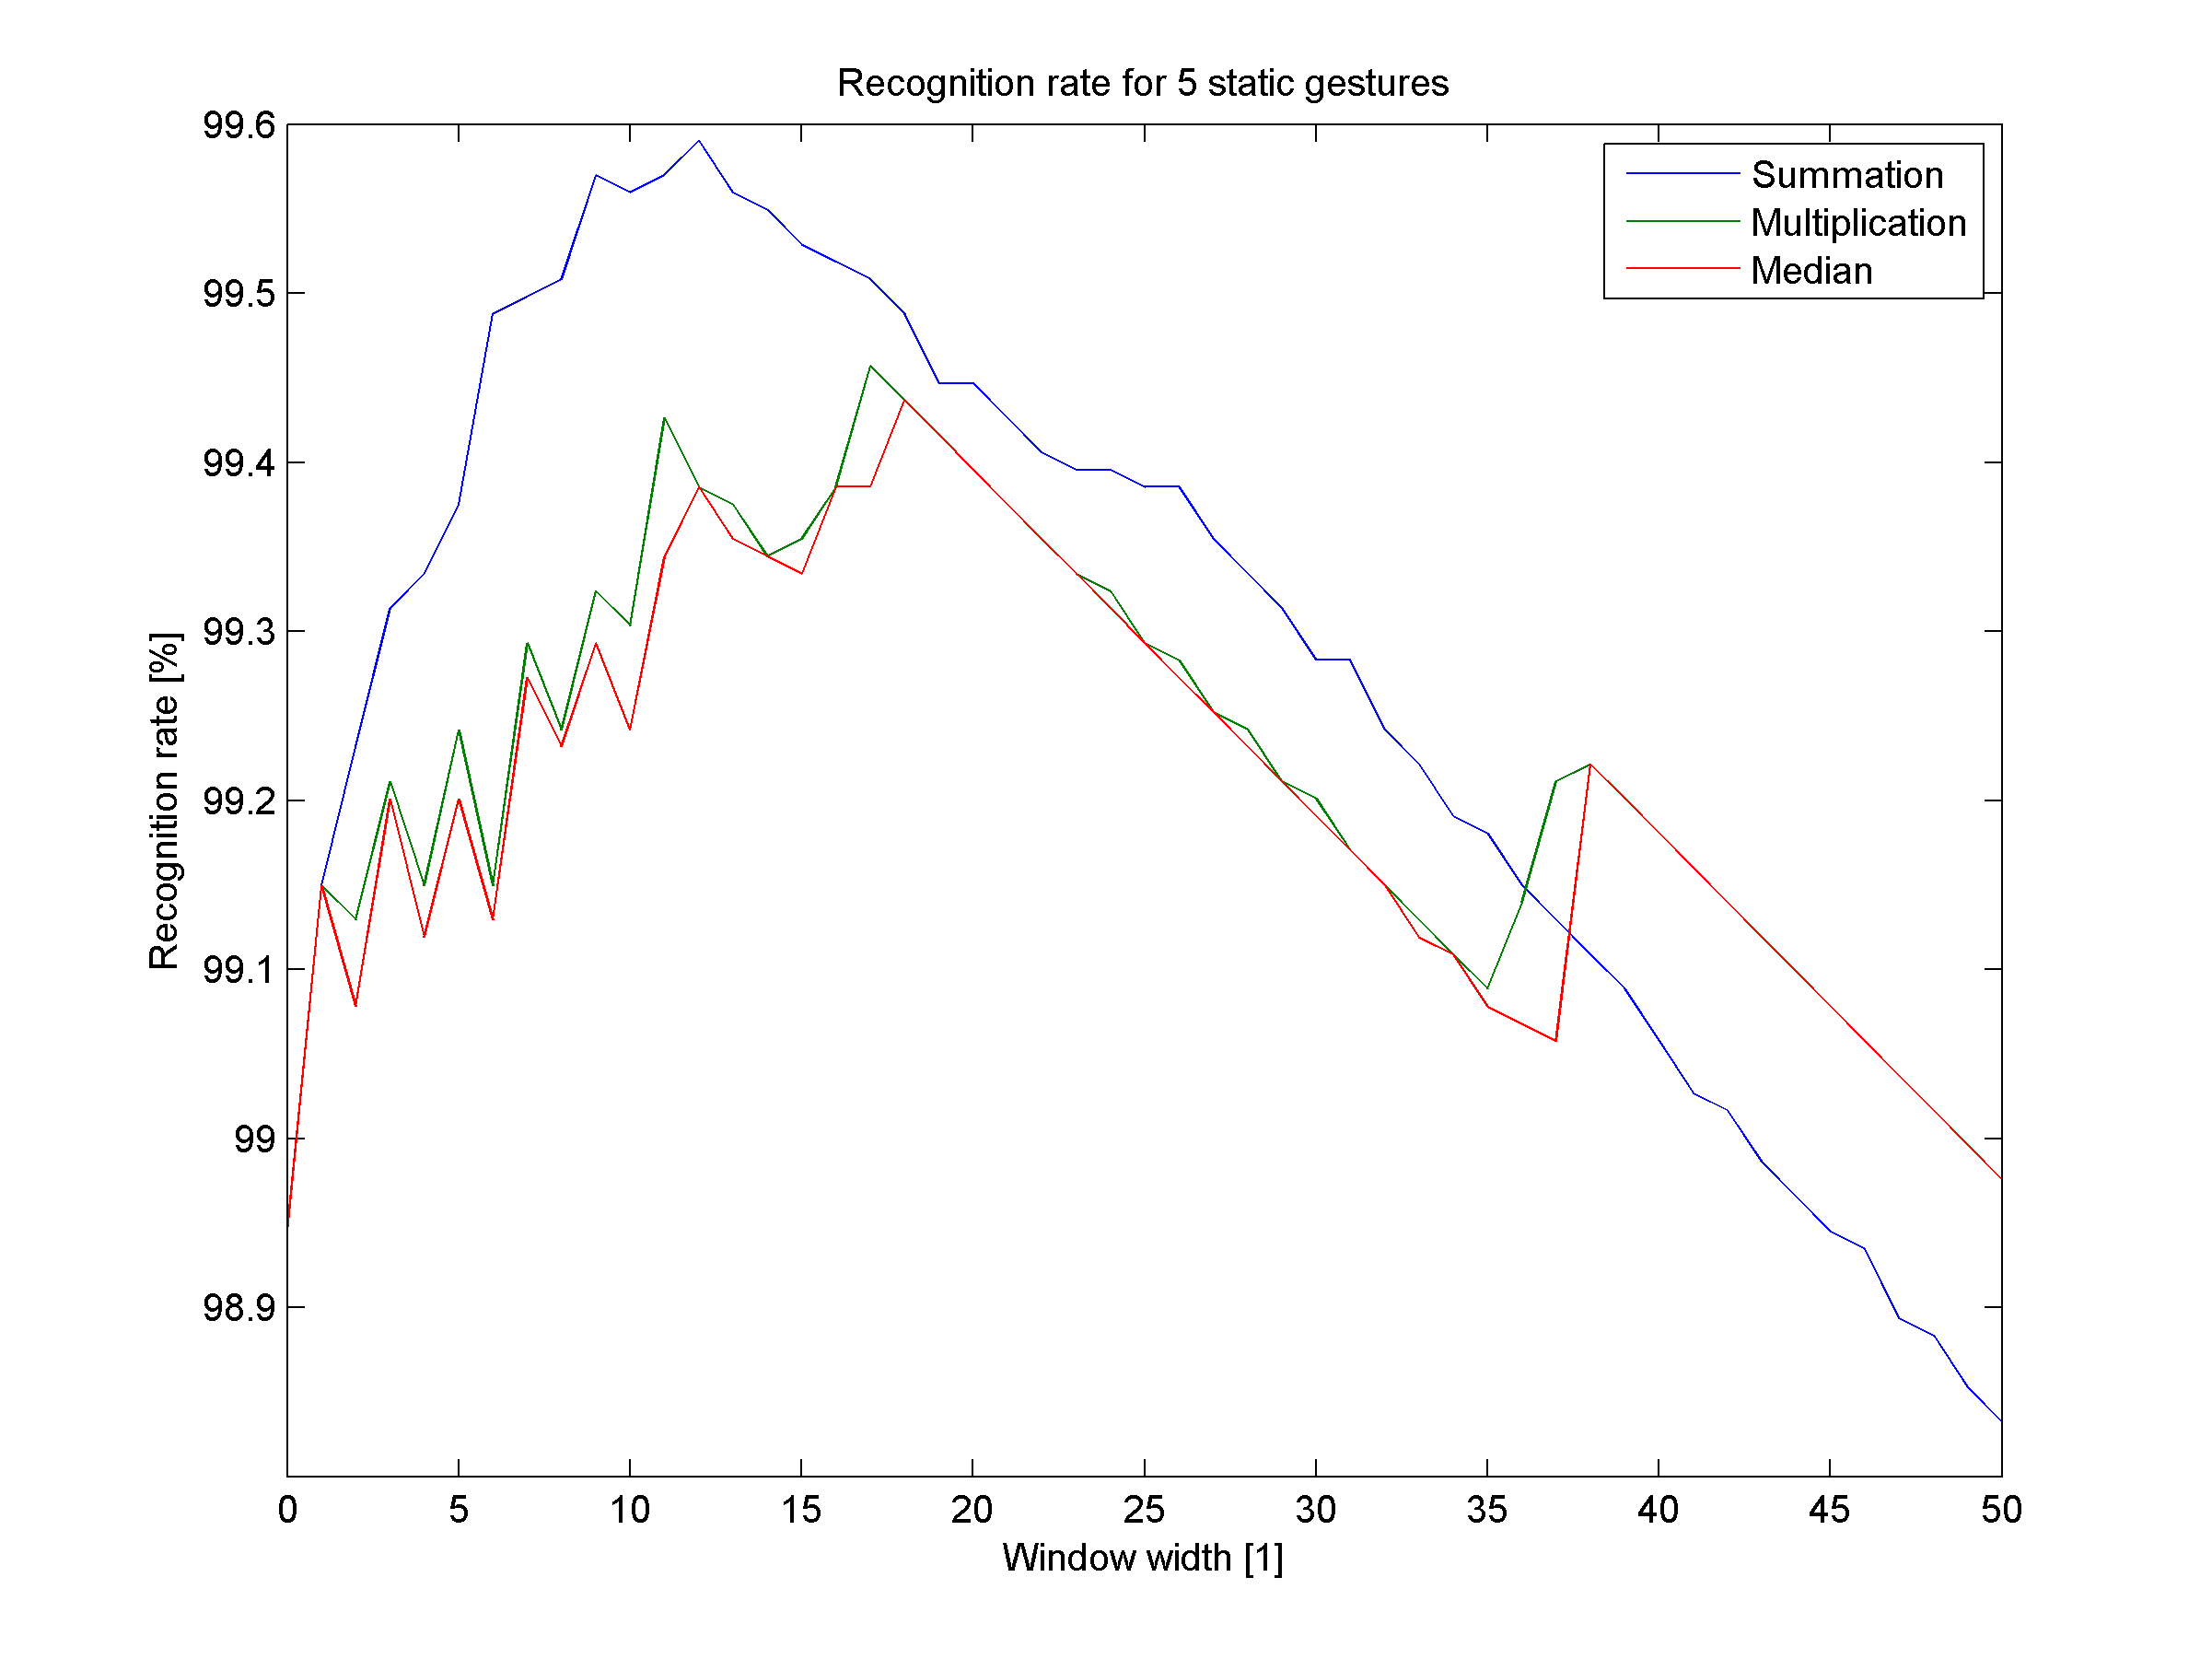
\includegraphics[width=0.5\textwidth]{figures/Mul5.png}
 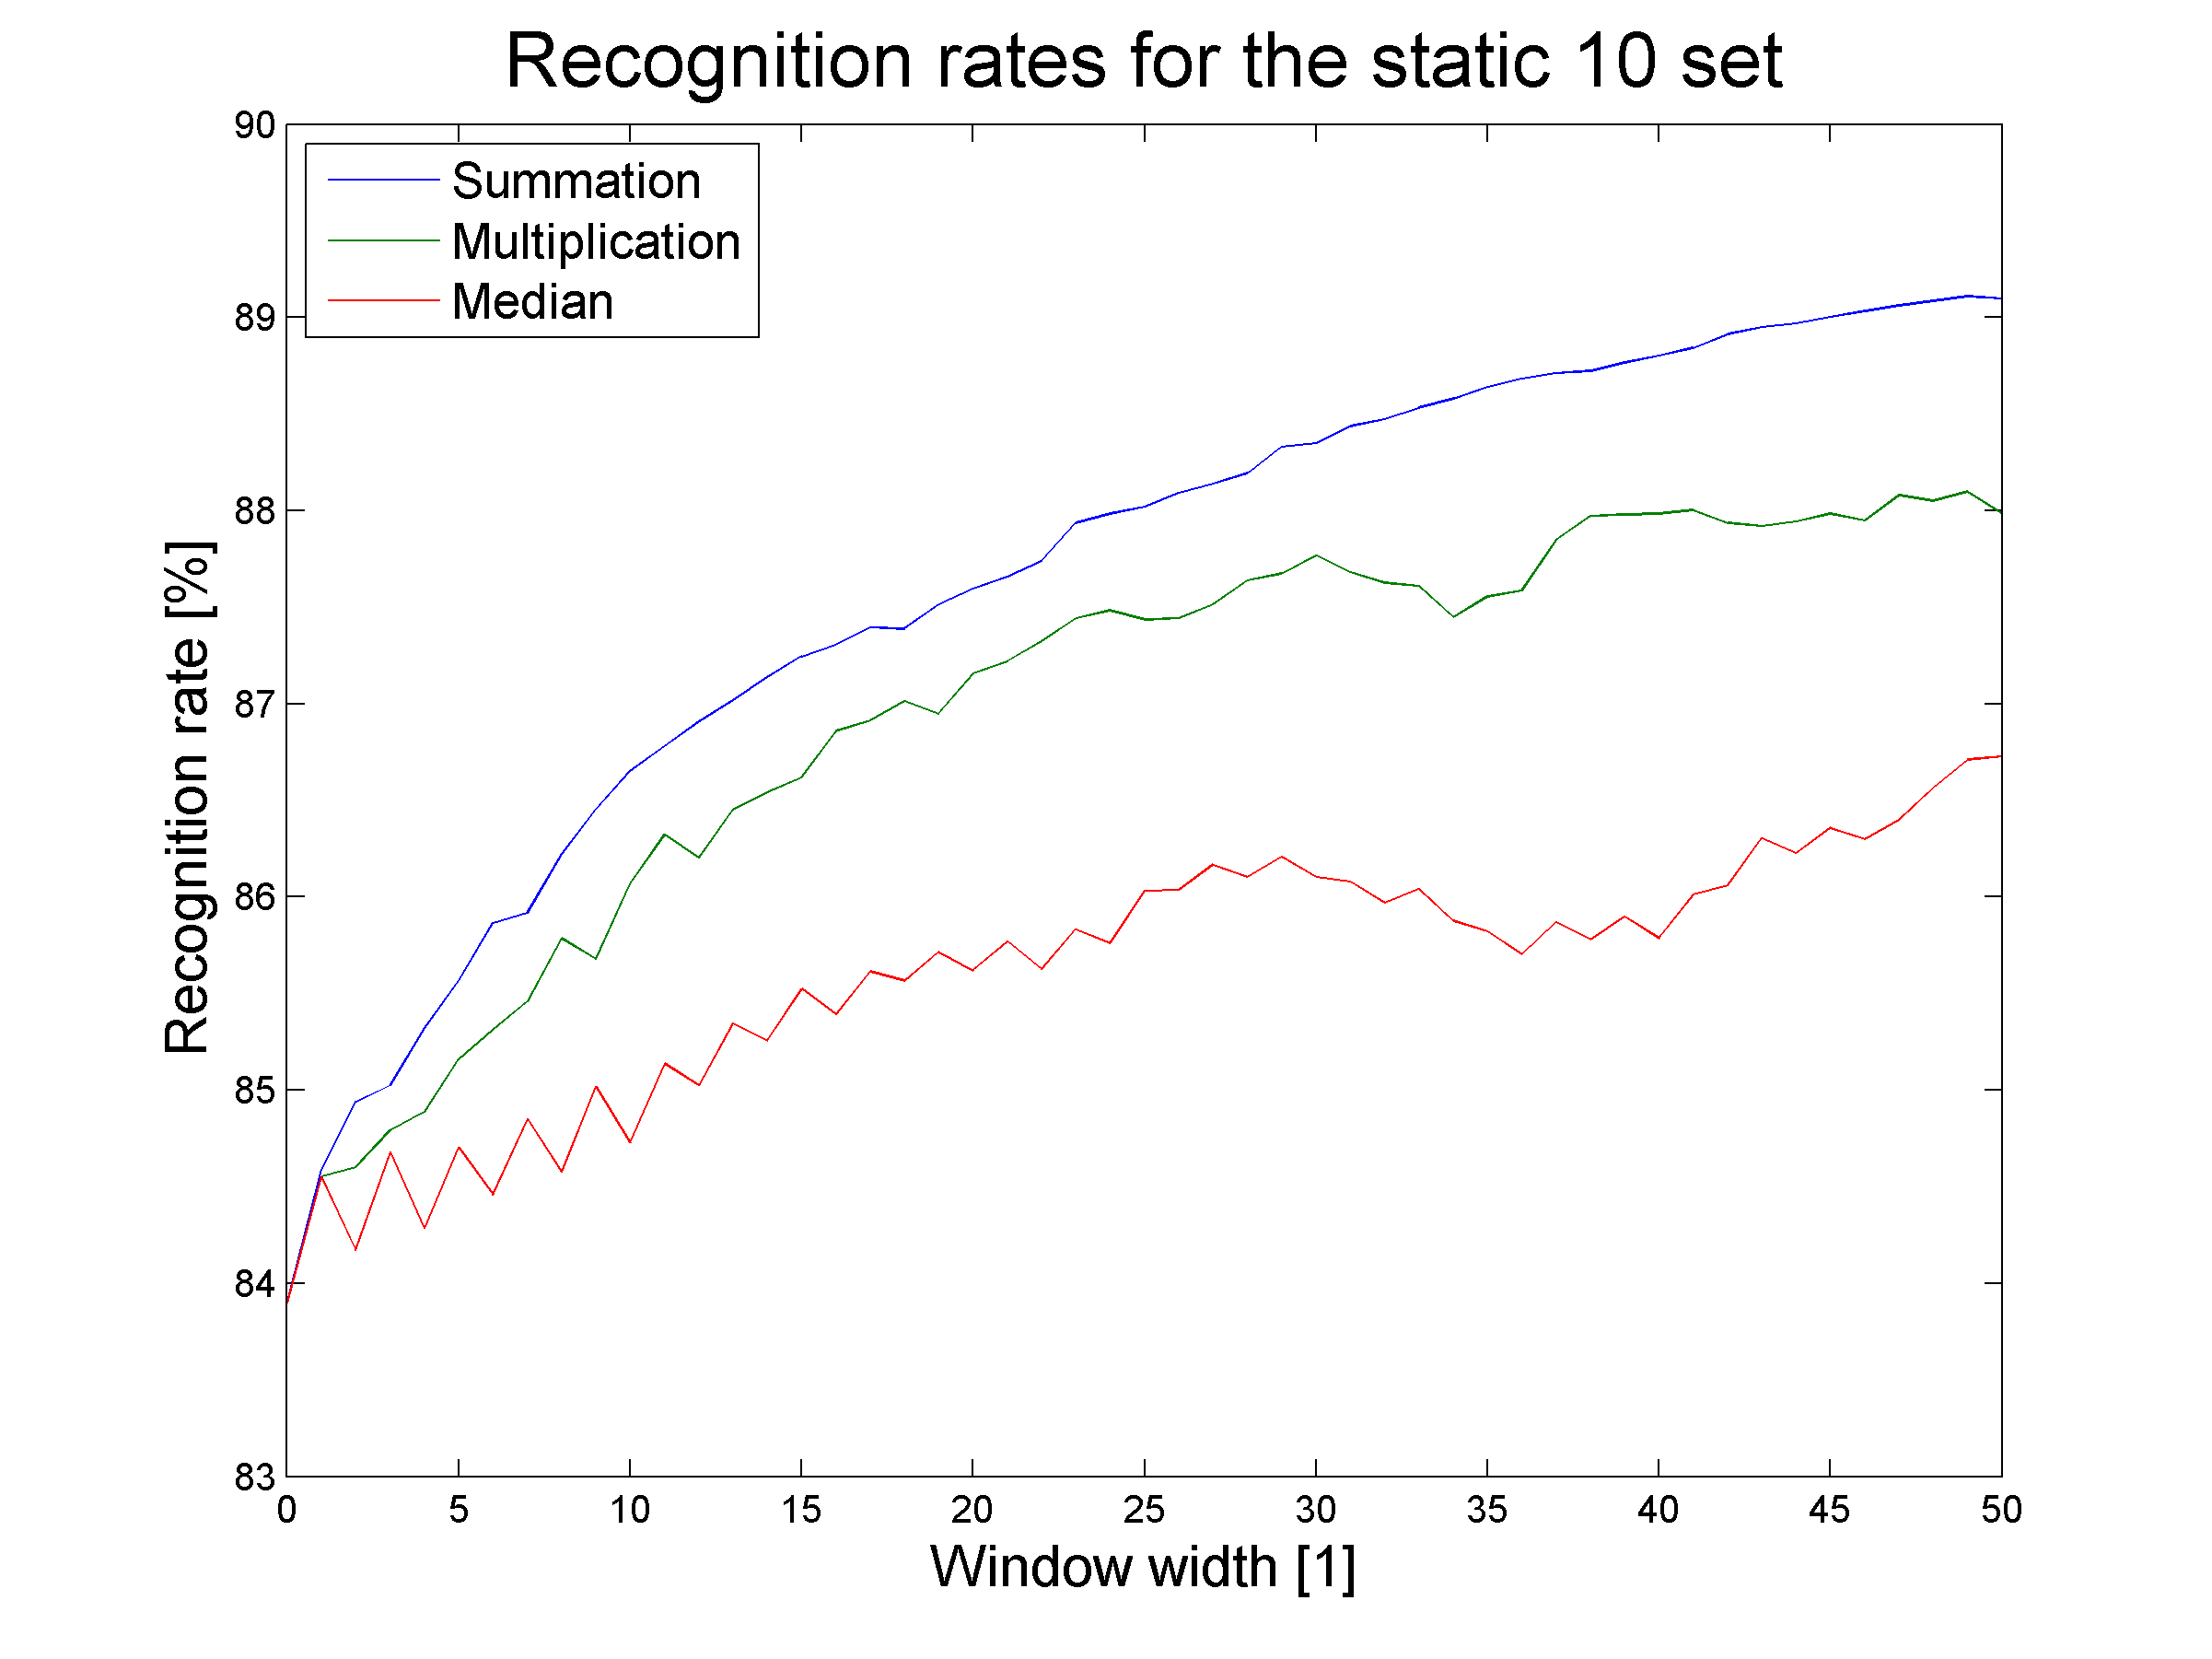
\includegraphics[width=0.5\textwidth]{figures/Mul10.png}
 }%
 \caption{Evaluation of different operators for result combining in case of different window sizes}
 \label{staticoper}
\end{figure}

 

The first approach to defining the sum operator is the operator of simple adding the elements of vectors $l$.
The second proposition is to multiple the corresponding elements of vectors $l$. 
The third approach utilizes the idea of calculating the median elements of vectors $l$.
The three approaches were compared for feature set 6, with preprocessing width equal to 10 for 5 and 10 gestures already used in previous experiments.
Simultaneously, the test were performed for different widths of window and are presented at fig.~\ref{staticoper}.
For almost all possible widths, the summation operator demonstrated the best recognition rate.
For 5 static gesture, the summation with width equal to 10 allowed to achieve the recognition rate over $99.5$\% gaining over $0.5\%$ when compared to solution without postprocessing.
Interestingly, windows wider than 12 resulted in lower recognition rate than the best achieved with window size equal to 10.
For 10 static gesture recognition problem, using window of size equal to 50 allowed to increase the recognition rate by over $5\%$ to the value over $89$\%.
In this case, wider window resulted in better results. 
Similarly to the preprocessing window size, also in postprocessing too wide window will result in delayed recognition rate of shown gesture.
Also, too wide window may result in worse results.
Therefore, the postprocessing window size of 10-15 is recommended, but it also depends on the application of the library.

With simple summation window, the currently achieved result and the results from the past are equally affecting the recognition result. 
Especially for wider windows, it can be assumed that the current measurement is more important than the measurement from the distant past.
That is why, the idea of weighted sum was introduced.
The weight distribution should have the highest weight for the current measurement and smaller values for results that were achieved earlier in time.

\begin{figure}[htb]
\centering

\centerline{%
 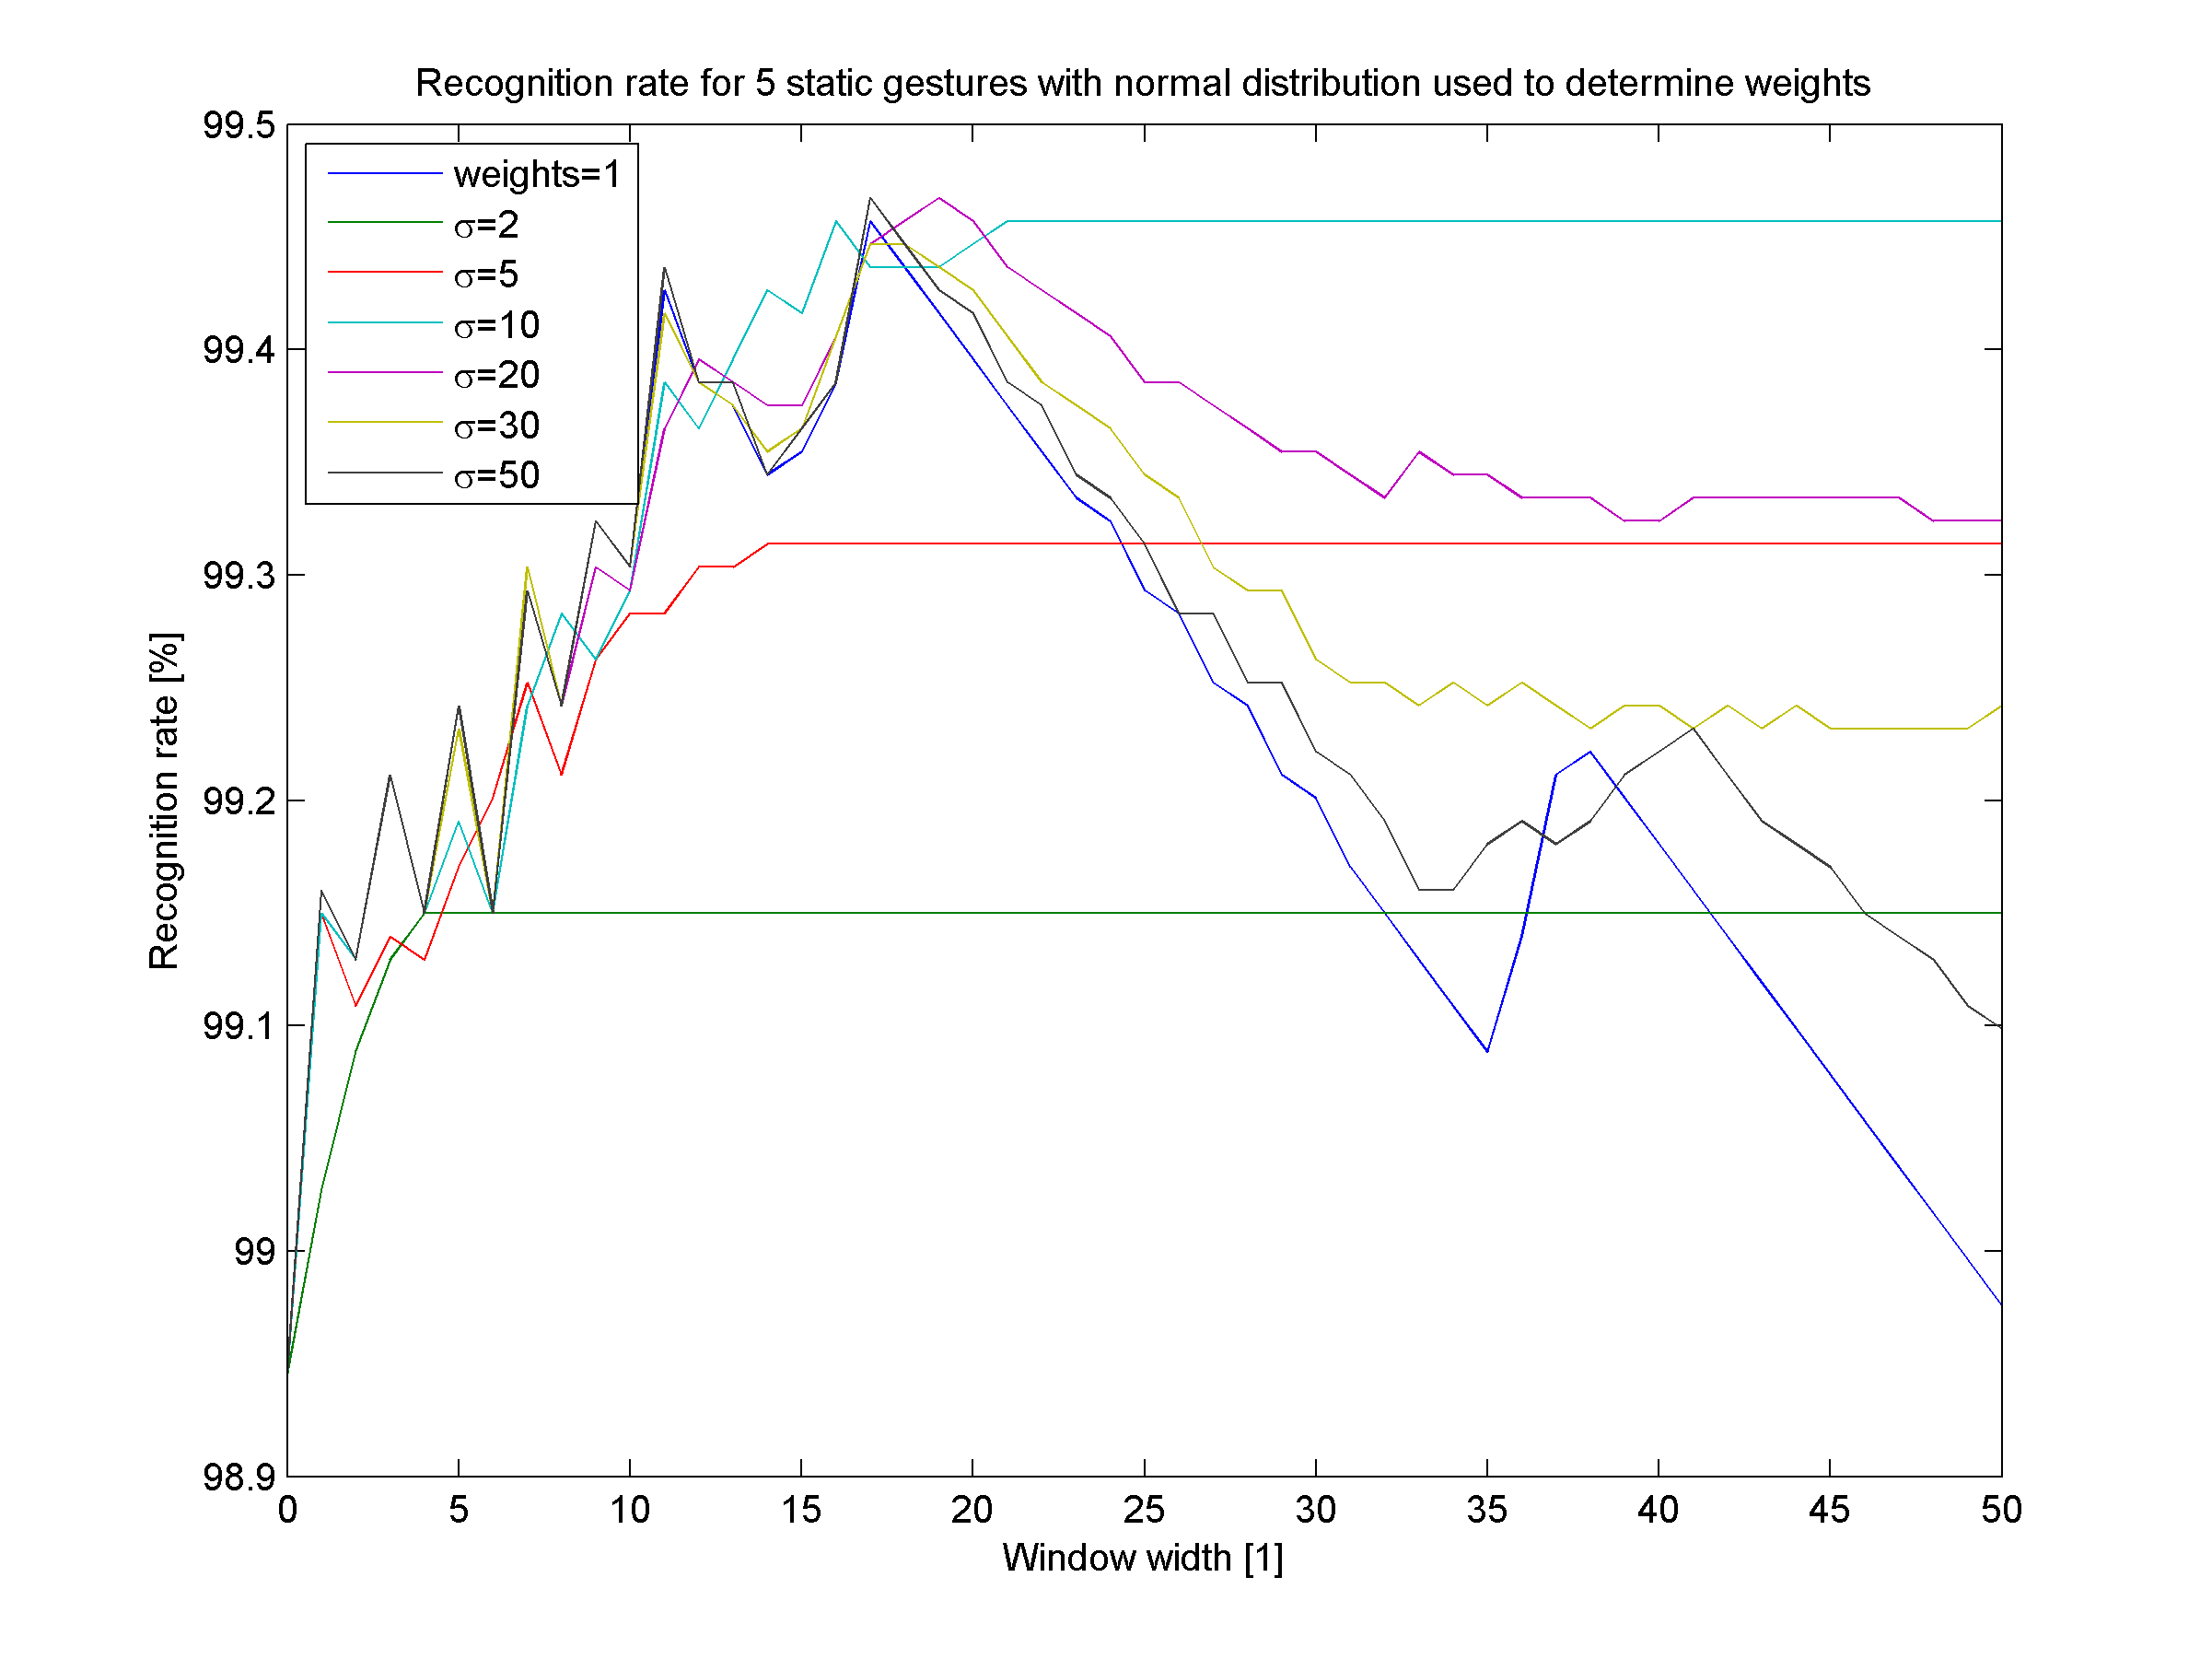
\includegraphics[width=0.5\textwidth]{figures/gaussSum5.png}
 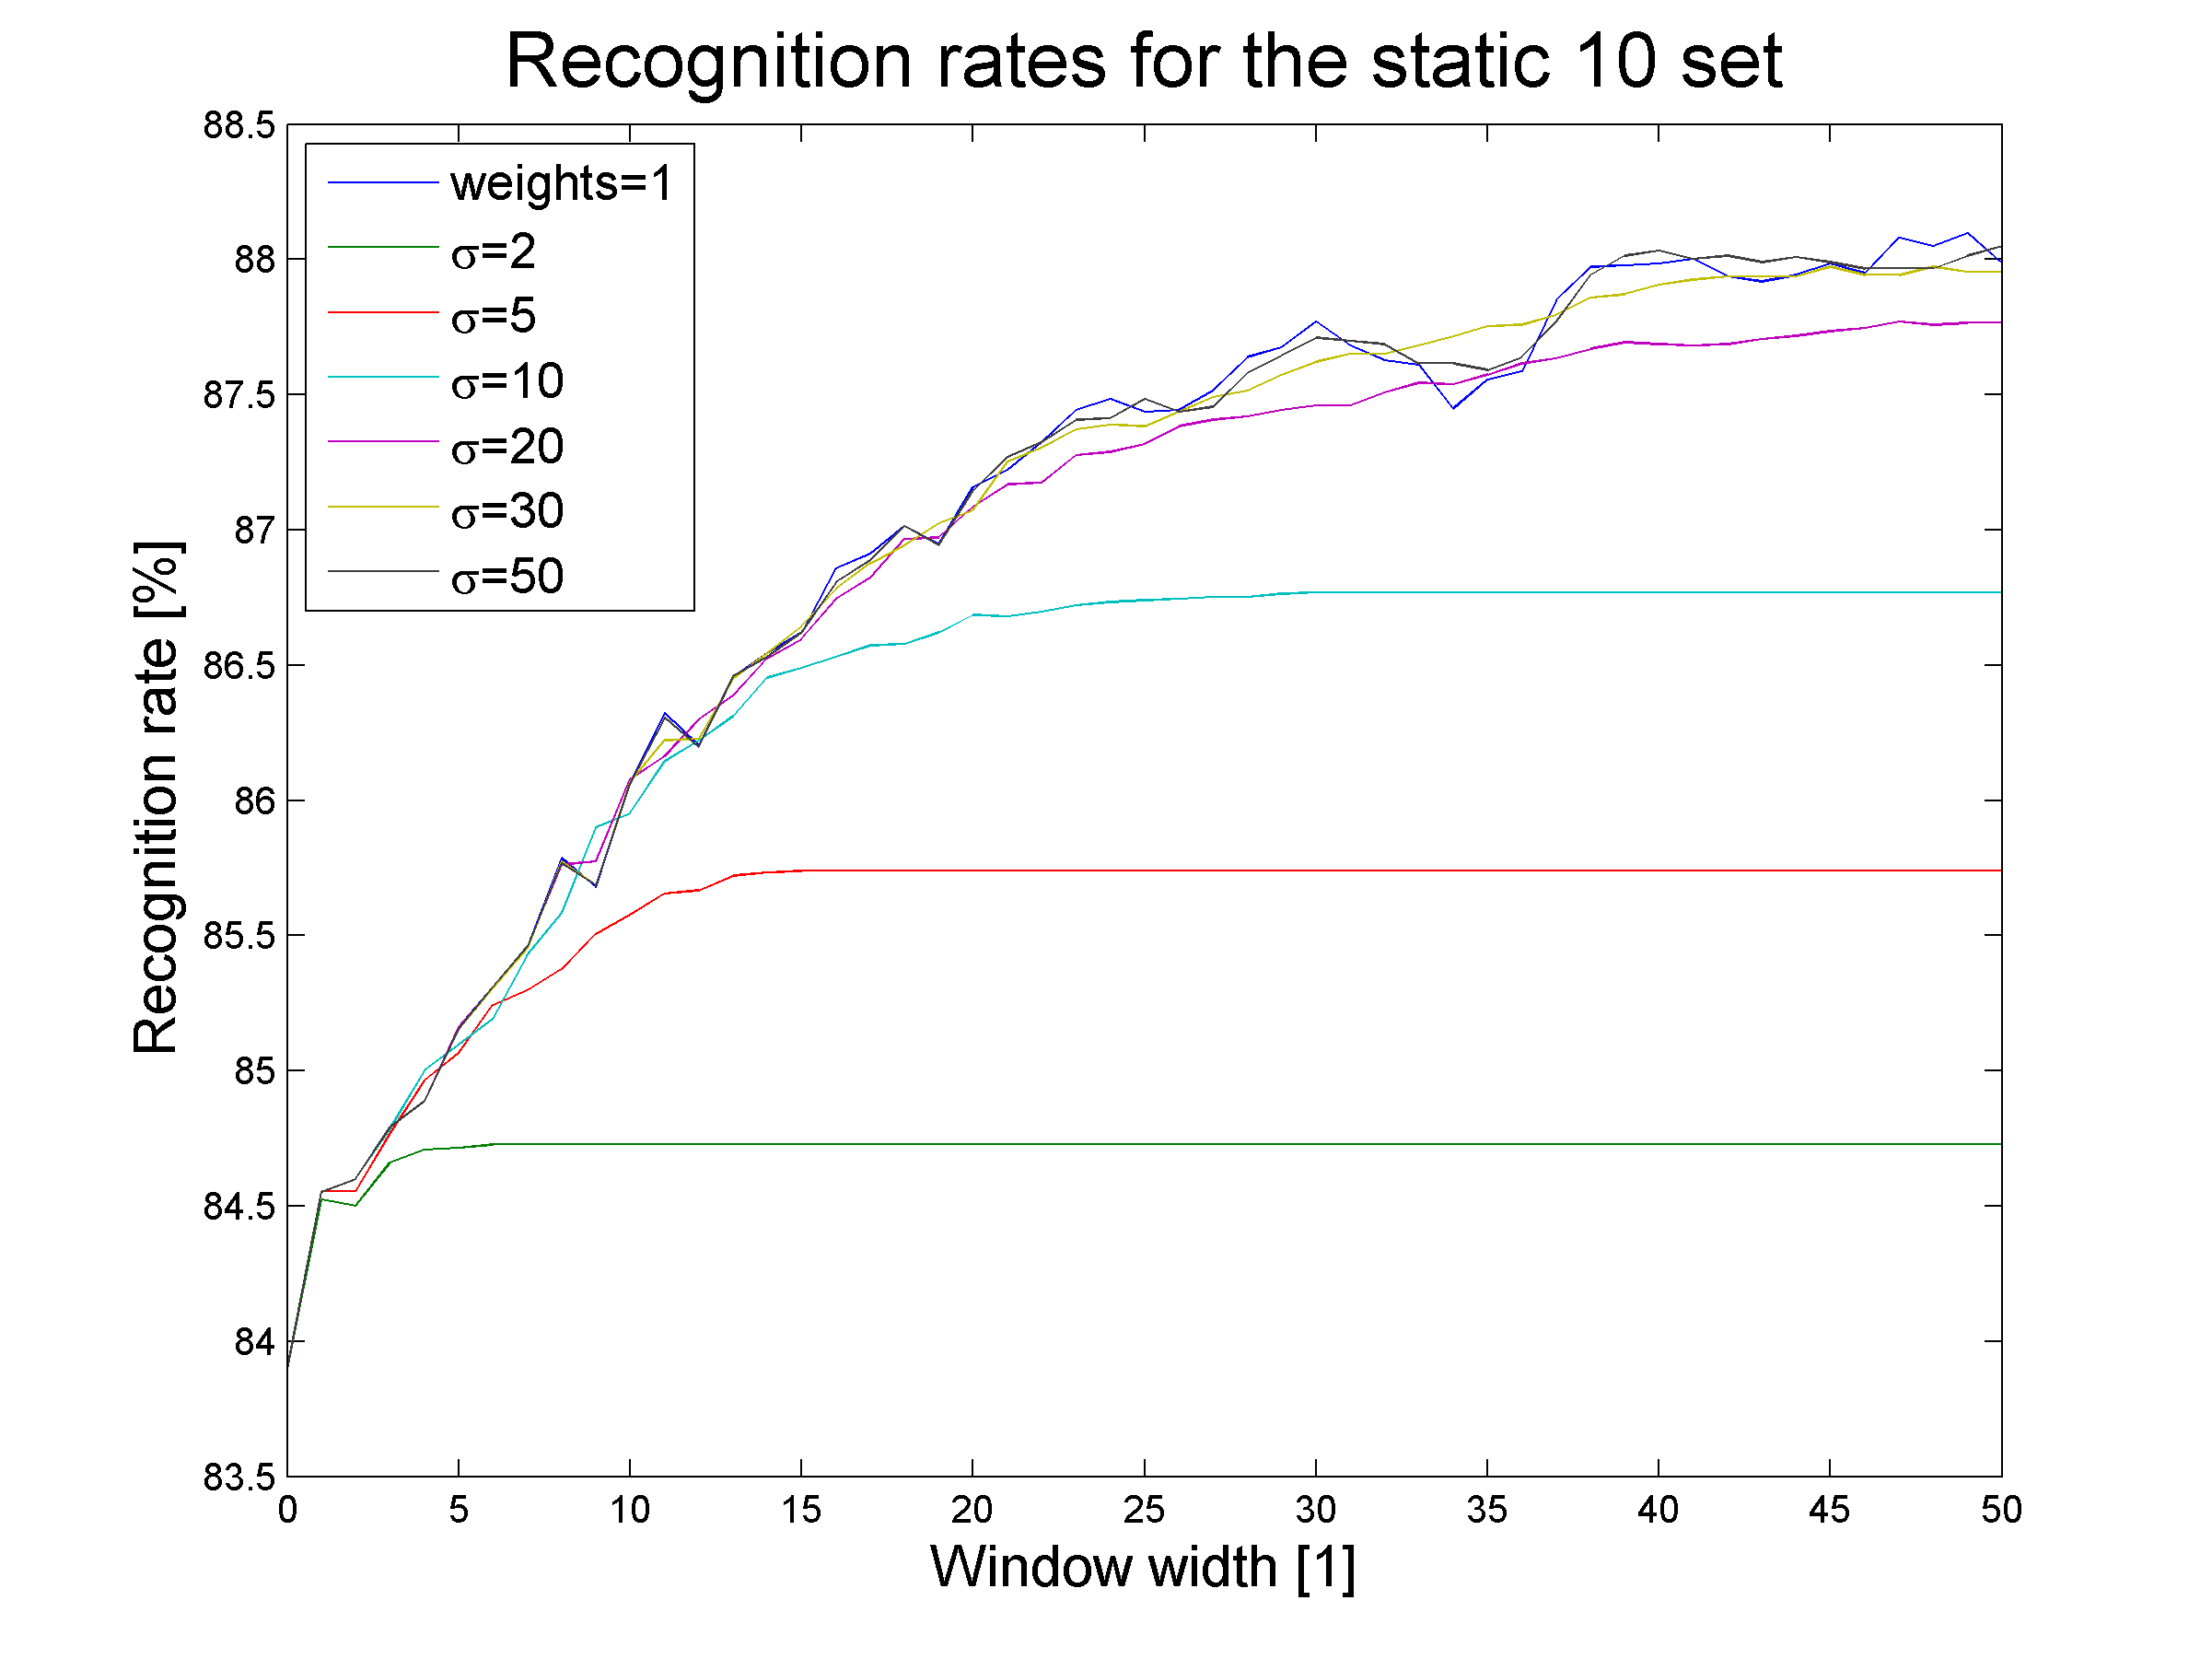
\includegraphics[width=0.5\textwidth]{figures/gaussSum10.png}
 }%
 \caption{Evaluation of weights for postprocessing distributed accordingly to normal distribution}
 \label{staticgauss}
\end{figure}

For this task, the half of the Gaussian distribution of weights can be used with maximal peak reached for the currently achieved result with weights slowly decreasing for measurements further away in time.
For Gaussian, the mean was assumed to be equal to $0$.
The standard deviation $\sigma$ was the parameter, which different values were tested.
The results were also performed for problems of recognition of 5 and 10 gestures.
The achieved results are presented in fig.~\ref{staticgauss}.
For 5 gestures, too small $\sigma$ prevented the increase of recognition rate due to the wider window size as the weights were equal to $0$. 
For greater sigmas, the achieved recognition rate is similar.
For this problem, the $\sigma$ equal to $10$ resulted in best recognition rate while the window was getting wider.
For problem of 10 static gesture recognition problem, greater sigma values achieved results comparable with the the results achieved with weights equal to 1.
As the usage of different weights also comes with greater computing cost and still did not result in better results, this part of processing can omitted without effecting the recognition.


From the presented results, the simple summation with uniform weights provides the greatest gain when it comes to the recognition rate and is the method recommended by the authors.


\section{Finger differentiation} 
Finger differentiation module is responsible to verify which particular fingers are detected during gesture recognition. The module can be used for additional processing on the user side, for which the information about the visible fingers can often be significant, It can also assist interpretation of data derived from parametrized gestures. The user can also use the module to better fit dataset features to the characteristics of selected gestures.
\subsection{Methods}
For this module were used the same classification algorithms (kernel functions) as those who had the best results in static gesture recognition. As in the case of static gesture recognition libSVM library has been used and RBF kernel has been selected.
\subsection{Evaluation methodology}
In the assumptions for static gesture recognitions was mentioned that the process must be independent of the position, rotation, sizes of hand and fingers. This presumption applies also to finger differentiation. However, this assumption is still does not contain one element, from which the differentiation process should be independent -- arrangement of hand. Whether forefinger is straight or bent, it is the same class, where only this one finger is taken out.

\subsubsection{Recorded dataset}
Dataset was collected by two different people. Each of them has recorded 32 classes, which reflect all the possible permutations of hand arrangements. The next step was to select from 32 gestures, those which are most frequently used by people in everyday life. Those 15 selected gestures are natural for human and do not cause a pain. People uses them as specific signes like peace sign. From the dataset were created four data collections used in the experiments:
\begin{itemize}
\item 32 gestures recorded by two people,
\item 15 gestures recorded by two people,
\item 32 gestures recorded by one person,
\item 15 gestures recorded by one person.
\end{itemize}

\subsection{Features}
As mentioned previously, it is important that the fingers differentiation process is independent of things like position of hand or size of finger. 

\begin{figure}[htb]
\centering
 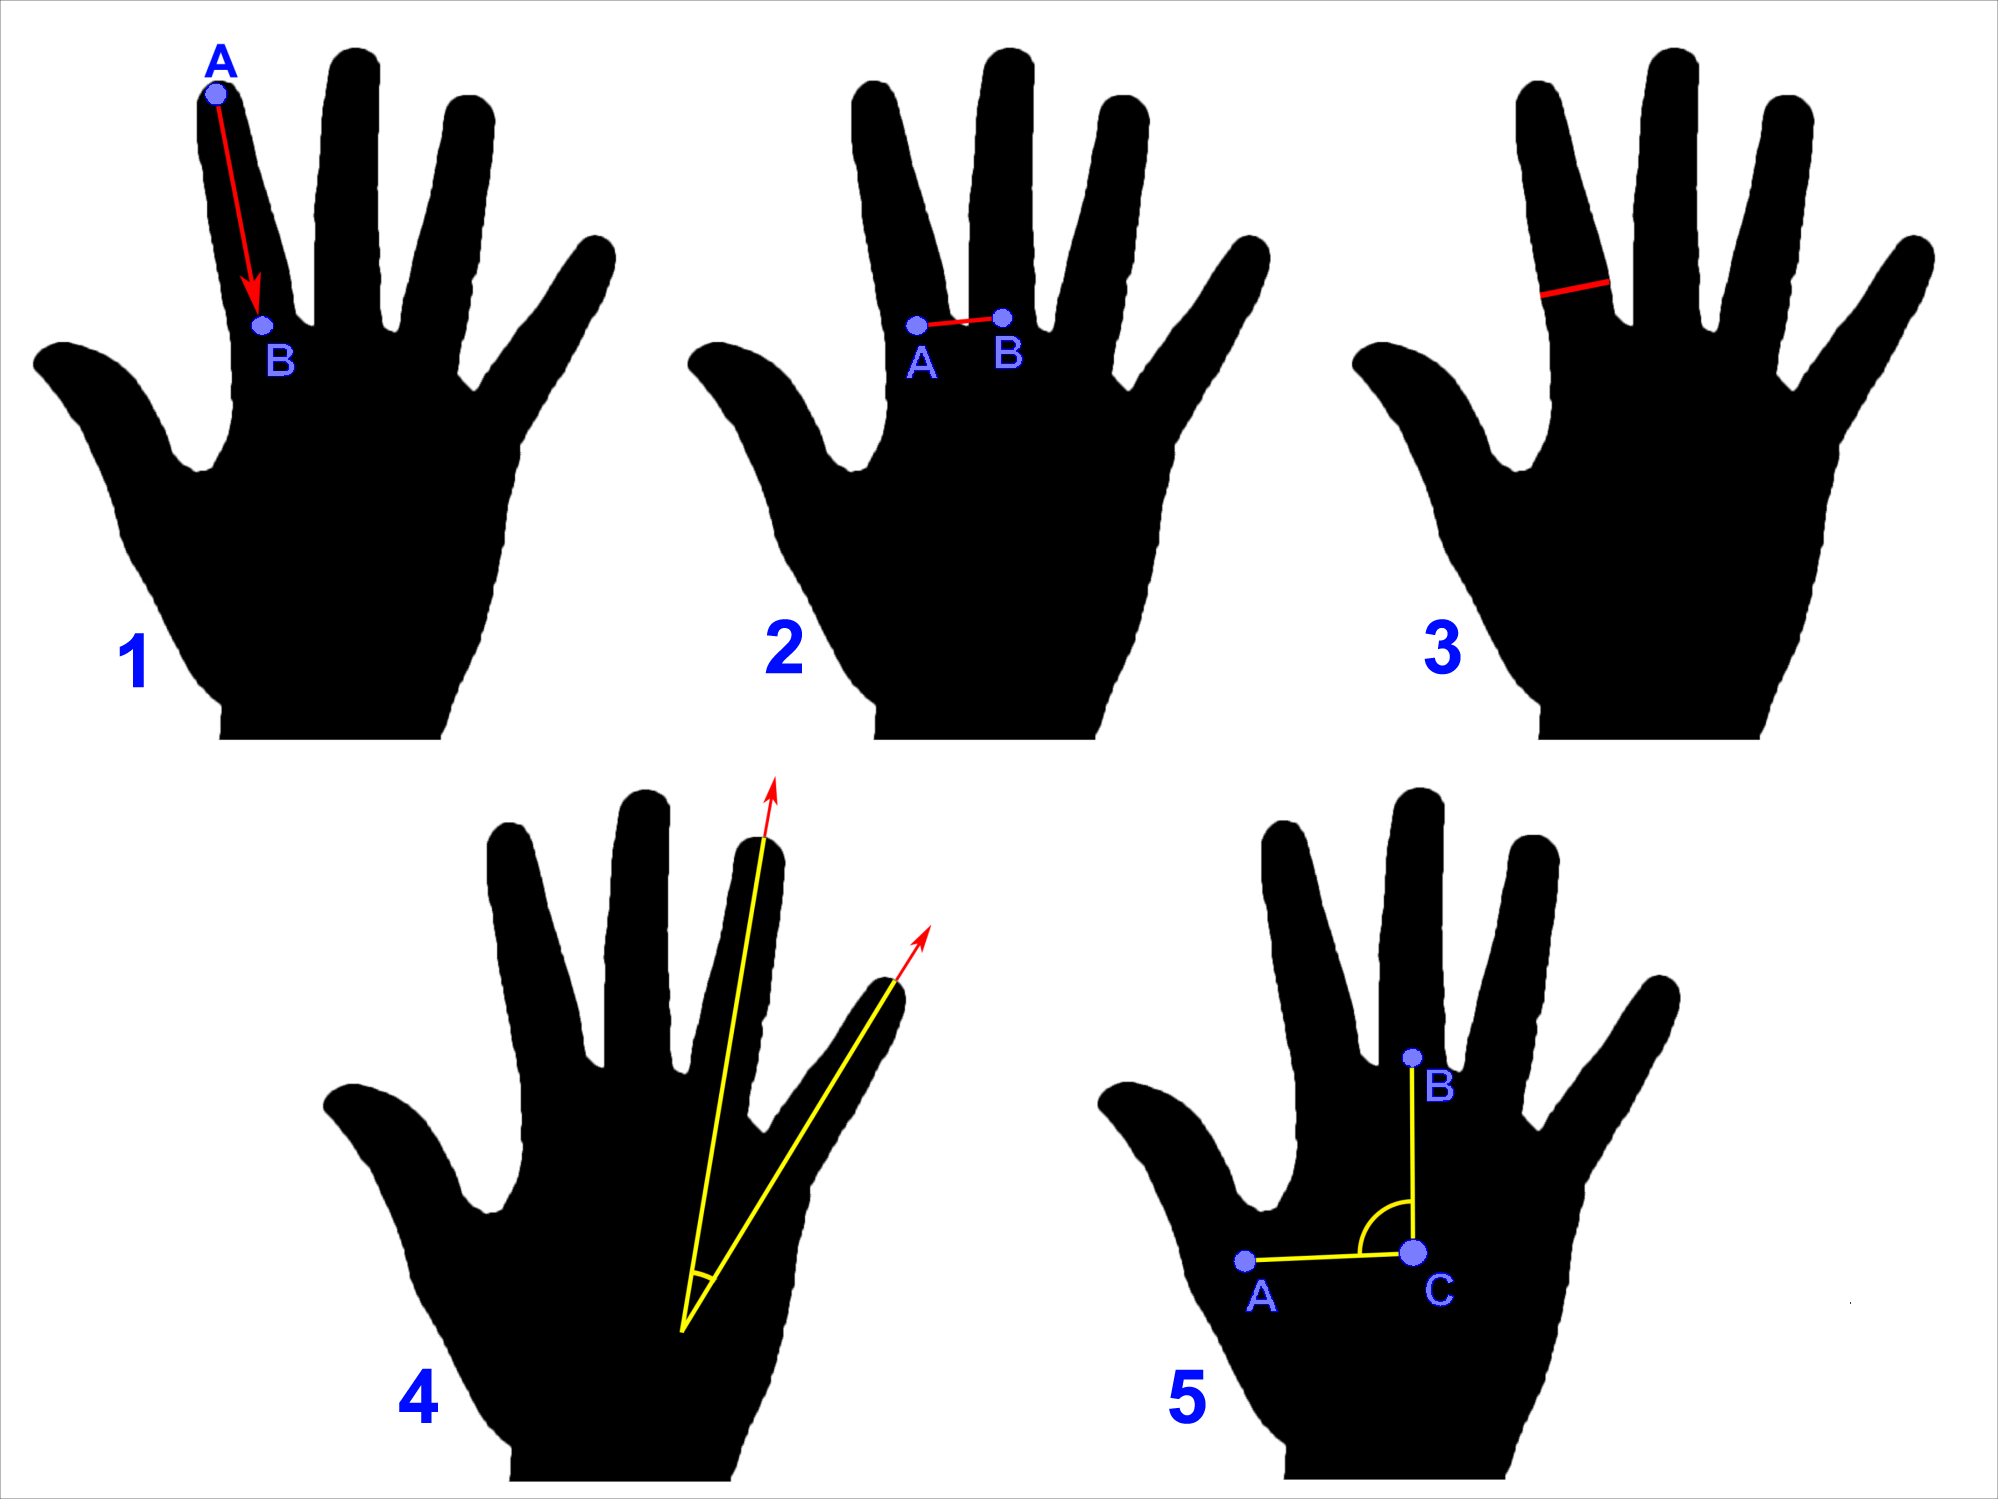
\includegraphics[width=0.75\columnwidth]{figures/fingDiffFeatures.png}
 \caption{Features used for finger differentiation}
 \label{fingfifffeatures}
\end{figure}

6 features were selected, which are independent of those parameters: 
\begin{enumerate}
\item finger count, 
\item distance between two nearest base points of a finger, 
To appoint a finger base point has to be reversed normalized direction vector multiplied by the length of a finger. Subsequent as the beginning of the vector thus formed is set finger tip position. The end of the vector indicates the finger base point (fig.~\ref{fingfifffeatures}.1). An example of distance between two nearest base points of a finger is showed on fig.~\ref{fingfifffeatures}.2.
\item ratio of the finger thickness to the maximal finger thickness, 
Leap Motion controller can return information about the thickness of the fingers (fig.~\ref{fingfifffeatures}.3). There are known relationships between the thicknesses of the fingers, for example that the thumb is the thickest finger. Just like in the previous feature ratio was used in order to become independent of size.
\item angles between two nearest fingers, 
In fig.~\ref{fingfifffeatures}.4  this feature has been shown. It is obtained by calculating the angle between the direction vectors of two adjacent fingers.
\item angles between finger and first finger relative to palm position. 
To calculate this angle three positions are needed : two finger tip positions and a palm position. The next step is to determine the line segments between palm position and finger tip positions. The searched angle is between two designated segments. This angle is marked in fig.~\ref{fingfifffeatures}.5.
\end{enumerate}

During testing new feature was created based on the features 2:\newline
2b. ratio of distance between two nearest base points of a finger to the minimal (non-zero) distance between two nearest base points
This feature is very similar to the previous one. The difference is that in this case is used ratio of distance and not the actual values. Thanks to this feature is independent of the size of hand.

\section{Experiments}
For the tests created several combinations of previously described features:
\begin{itemize}
\item 1,2,4
\item 1,3,5
\item 1,3,4,5
\item 1,2,3,4,5
\end{itemize}

All sets of features has been tested for all four datasets. The percentage results can be seen in table~\ref{findiff}. From the data obtained it can be concluded that the best match is when the all features are used. However, feature 2 is not independent of the size of the hand. Therefore, a new feature has been created using the ratio of two values obtained from the original feature. Then the test was performed for a set of: 1, 2b, 3, 4, 5 for all the dataset. The result for this test is in the last line of the table~\ref{findiff}. Interestingly, despite the fact that the modified feature is independent of the size of hand, attribute 2b had an inferior result than the original feature, which operates on the actual value of the distance apart fingers. 

\begin{table}[htp!]
\begin{center}
	\label{findiff}
	\caption{Results obtained by experimental feature sets for different data collections}
    \begin{tabular}{|c|c|c|c|c|}
    \hline
    features & 32 classes, 2 people & 15 classes, 2 people & 32 classes, 1 person  & 15 classes, 1 person  \\ \hline
    1,2,4		& 75.393\% & 87.288\%  & 78.411\% & 90.608\% \\ \hline
    1,3,5              	& 76.291\% & 87.504\%  & 79.638\% & 91.548\% \\ \hline
    1,3,4,5            	& 78.082\% & 87.504\%  & 79.638\% & 91.548\% \\ \hline
    1,2,3,4,5           & 83.180\% & 90.278\%  & 85.825\% & 93.036\% \\ \hline
    1,2b,3,4,5          & 76.553\% & 87.619\%  & 79.798\% & 91.629\% \\ \hline
    \end{tabular}
    \end{center}
\end{table}

It is worth to mention that it seemed that feature 4 -- angles between two nearest fingers -- will have a substantial contribution to finger differentiation. However, the results showed that this feature has impact only on the largest amount of data, while in other cases brought nothing.

In the second round of tests was verified how preprocessing will affect the finger differentiation process. For the best set of features from the previous test was performed a new test with preprocessing for all datasets. 

\begin{table}[htp!]
\begin{center}
	\label{findiffpre}
	\caption{The recognition rate achieved with feature set 1,2,3,4,5}
    \begin{tabular}{|c|c|c|c|c|}
    \hline
    features & 32 classes, 2 people & 15 classes, 2 people & 32 classes, 1 person  & 15 classes, 1 person  \\ \hline
    1,2,3,4,5           & \% & \%  & \% & \% \\ \hline
    \end{tabular}
    \end{center}
\end{table}


